\documentclass[tikz, border=10pt]{standalone}
%%%<
\usepackage{verbatim}
\usetikzlibrary{shapes}

\tikzset{
    vertex/.style = {
        circle,
        fill            = black,
        outer sep = 2pt,
        inner sep = 1pt,
    }
}
\begin{document}
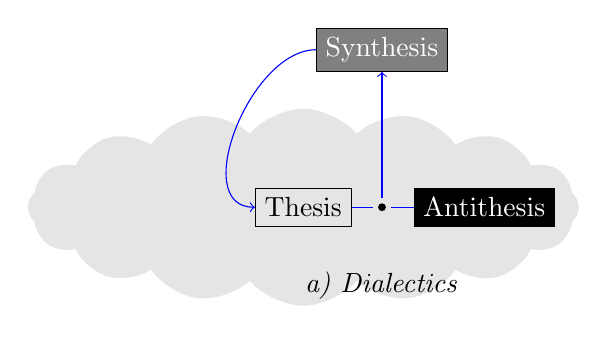
\begin{tikzpicture}
  % Dialectics
  
  \node[cloud, fill=gray!20, cloud puffs=16, cloud puff arc= 100,
        minimum width=7cm, minimum height=2.5cm, aspect=1] at (0,0) {};
  
  \node[draw] (Thesis) at (0,0) {Thesis};
  \node[draw,fill=black,text=white] (Antithesis) at (2.3,0) {Antithesis};
  \node[draw,fill=gray,text=white] (Synthesis) at (1,2) {Synthesis};
  
  \draw node[vertex] (Joint) at (1,0) {};
  
  \draw[-,draw=blue] (Thesis) to (Joint);
  \draw[-,draw=blue] (Antithesis) to (Joint);
  \draw[->,draw=blue] (Joint) to (Synthesis);
  \draw[->,draw=blue] (Synthesis) to[in=180,out=180] (Thesis);
  
  \node at (1.0, -1.0) {\textit{a) Dialectics}};
\end{tikzpicture}
\end{document}